\documentclass[aspectratio=169]{beamer}


\usepackage{fontspec}
\usepackage{polyglossia}
\usepackage{color}
\setdefaultlanguage{russian}

\usetheme{metropolis}

\metroset{background=light}
\metroset{sectionpage=none}
\metroset{numbering=fraction}

\definecolor{ssaublue}{RGB}{77,144,205}
\setbeamercolor{frametitle}{fg=white, bg=ssaublue}
\setbeamercolor{title separator}{fg=ssaublue}
\setmainfont[
    Path = fonts/elektratextpro/,
    Extension = .otf,
    UprightFont = elektratextpro,
    BoldFont = elektratextpro_bold,
    ItalicFont = elektratextpro_italic
]{elektratextpro}

\setsansfont[
    Path = fonts/elektratextpro/,
    Extension = .otf,
    UprightFont = elektratextpro,
    BoldFont = elektratextpro_bold,
    ItalicFont = elektratextpro_italic
]{elektratextpro}

\setmonofont[
    Path = fonts/elektratextpro/,
    Extension = .otf,
    UprightFont = elektratextpro,
    BoldFont = elektratextpro_bold,
    ItalicFont = elektratextpro_italic
]{elektratextpro}

\newfontfamily\cyrillicfont[
    Path = fonts/elektratextpro/,
    Extension = .otf,
    UprightFont = elektratextpro,
    BoldFont = elektratextpro_bold,
    ItalicFont = elektratextpro_italic
]{elektratextpro}

\newfontfamily\cyrillicfontsf[
    Path = fonts/elektratextpro/,
    Extension = .otf,
    UprightFont = elektratextpro,
    BoldFont = elektratextpro_bold,
    ItalicFont = elektratextpro_italic
]{elektratextpro}

\newfontfamily\cyrillicfonttt[
    Path = fonts/elektratextpro/,
    Extension = .otf,
    UprightFont = elektratextpro,
    BoldFont = elektratextpro_bold,
    ItalicFont = elektratextpro_italic
]{elektratextpro}

\title{Что такое DevOps?}
\author{Правдин Иван}
\date{24.05.2025}

\begin{document}
    \maketitle

    \begin{frame}{О чем этот курс?}
        \begin{itemize}
            \item Знакомство с популярными практиками в промышленной разработке ПО
        \end{itemize}
    \end{frame}

    \begin{frame}{О чем этот курс?}
        \begin{figure}
            
\includegraphics[width=1\textwidth]{images/spectrum}
        \end{figure}
    \end{frame}

    \begin{frame}{О чем этот курс?}
        \begin{itemize}
            \item Обзор DevOps инструментария и его применение на практике
        \end{itemize}
    \end{frame}
    {
        \setbeamertemplate{frame footer}{
            \scriptsize\href{https://digital.ai/learn/devsecops-periodic-table}{\textcolor{lightgray}{https://digital.ai/learn/devsecops-periodic-table}}
        }
        \begin{frame}{О чем этот курс?}
            \begin{figure}
                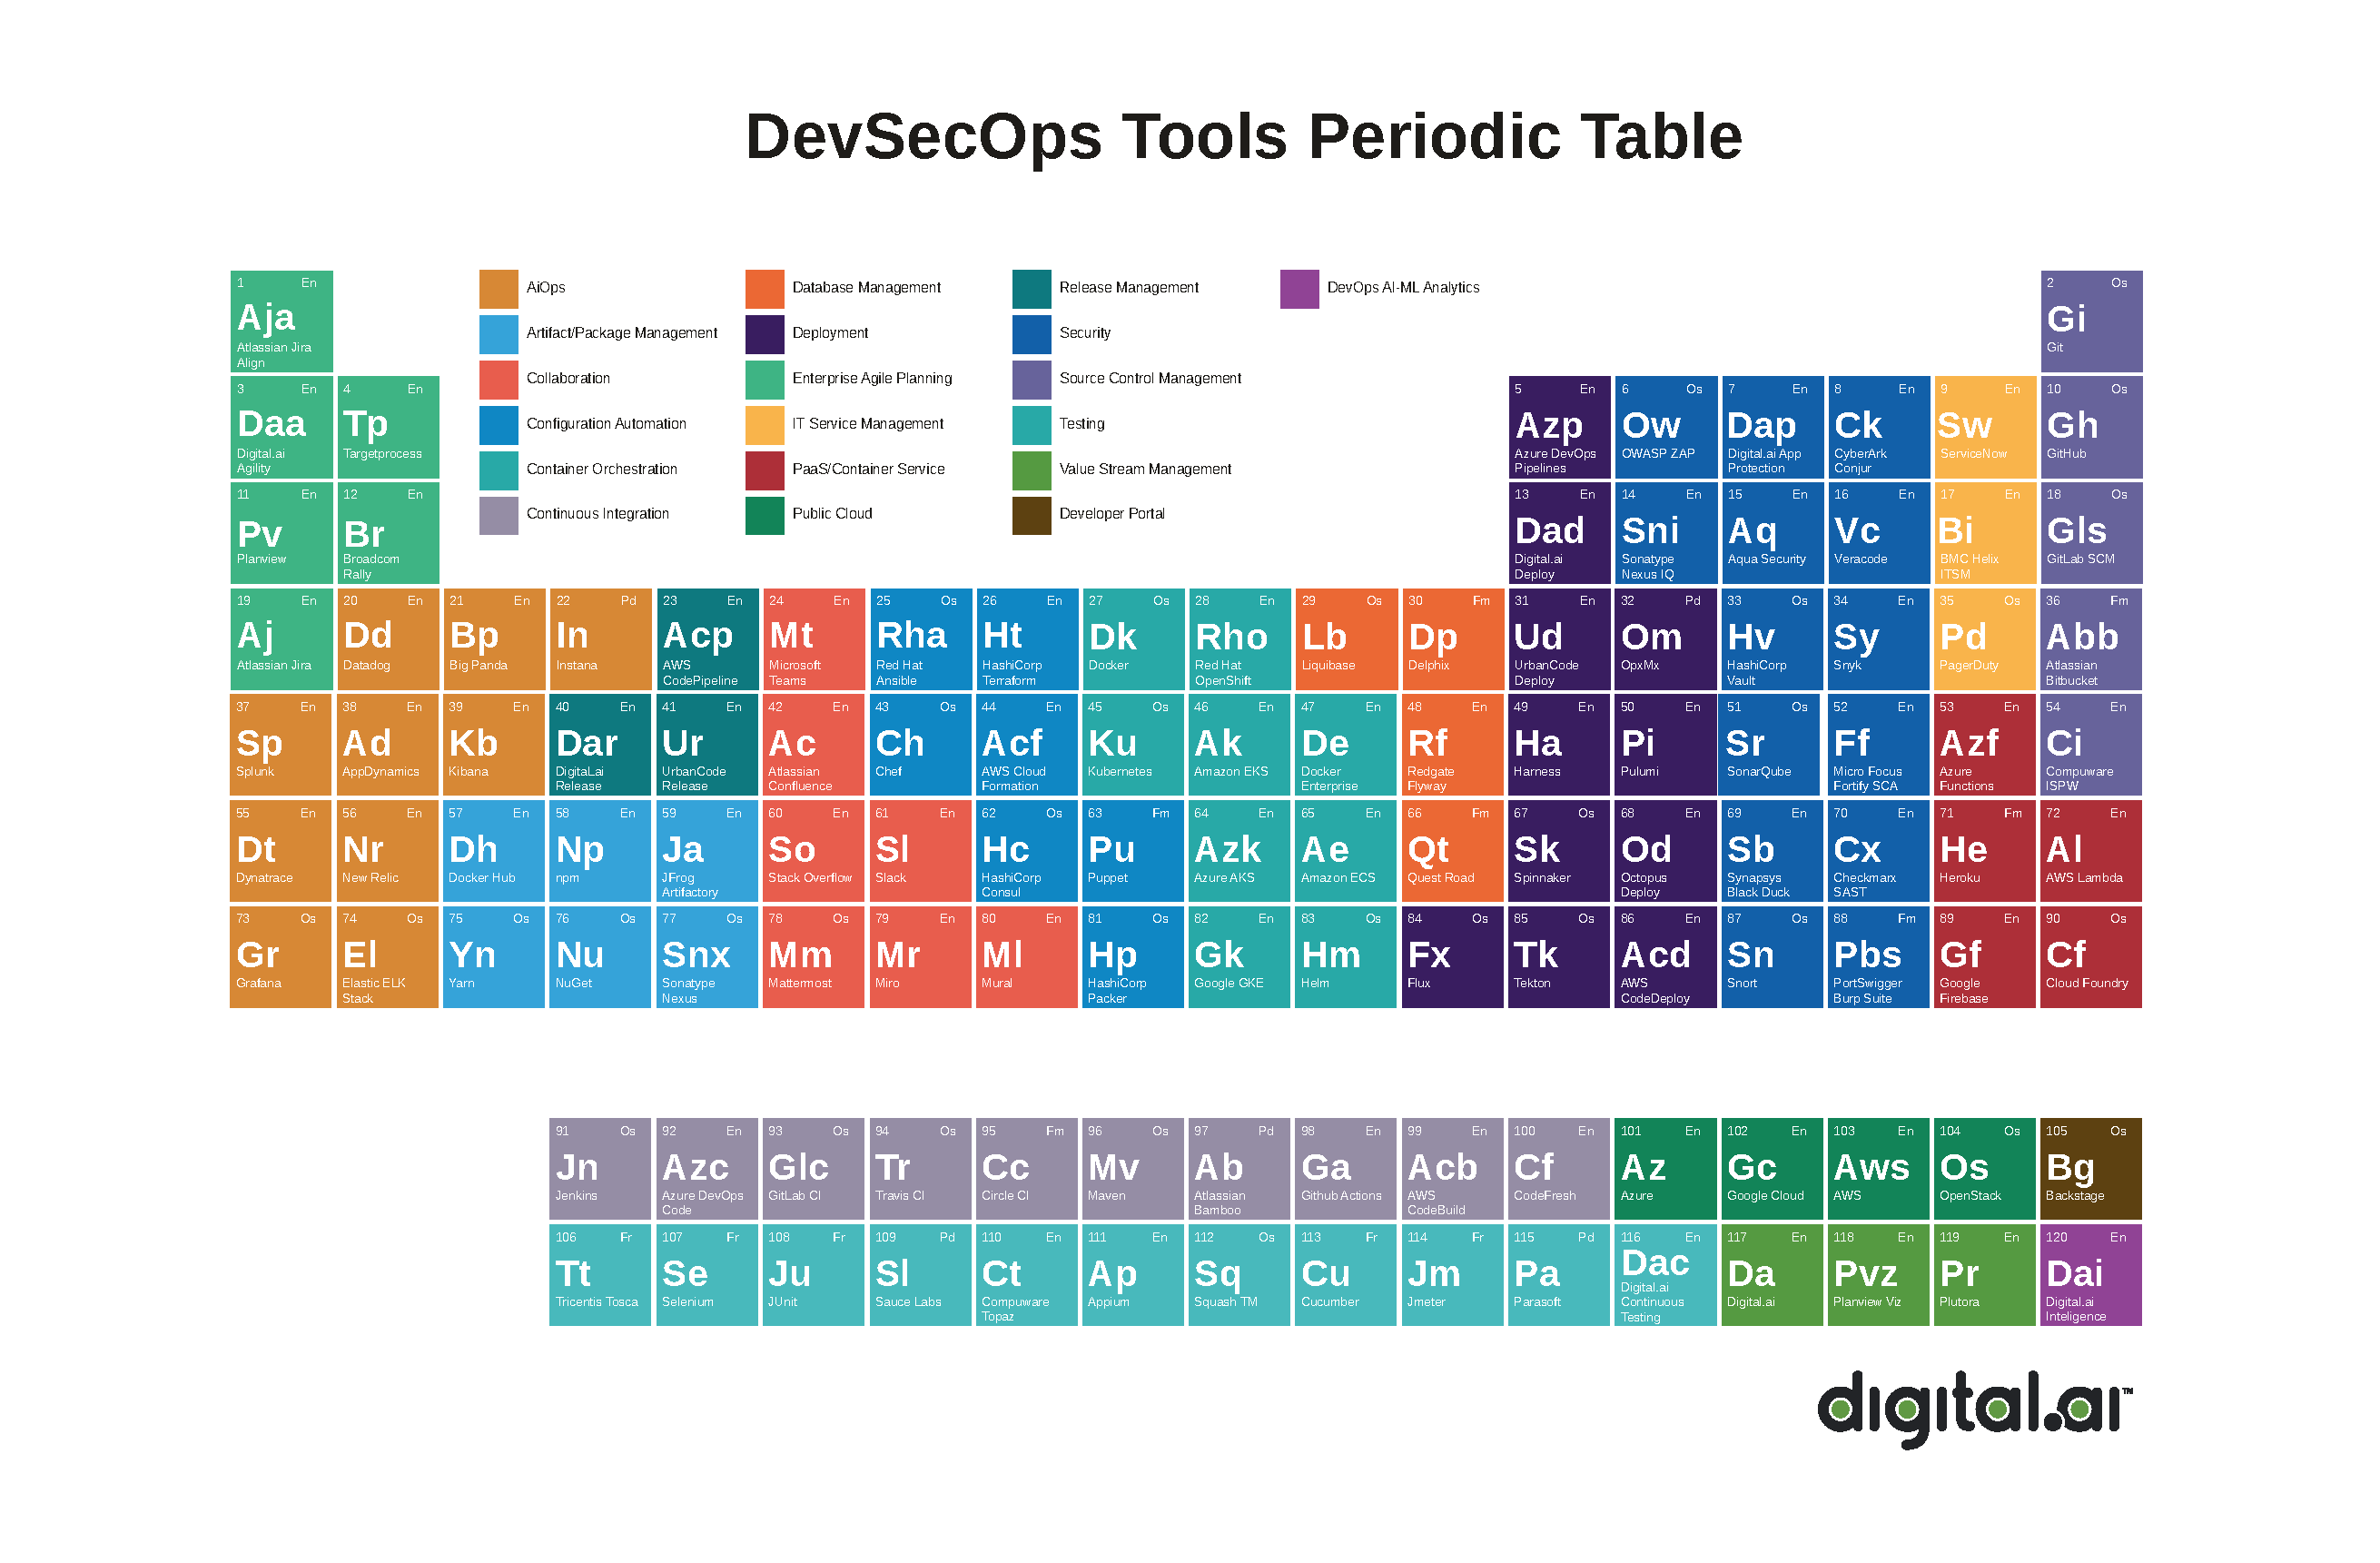
\includegraphics[width=0.8\textwidth]{images/digital-ai-periodic-table-of-devsecops-2025-March}
            \end{figure}
        \end{frame}
    }

    \begin{frame}{План курса}
        \begin{itemize}
            \item Введение в проблему
            \item Технические методы и инструменты для реализации практик DevOps
            \item CI/CD пайплайн и его ключевые компоненты
            \item Среды выполнения кода и их конфигурация
            \item Continuous Delivery системы
            \item Deployment стратегии
            \item Сопутствующие системы при разработке ПО
        \end{itemize}
    \end{frame}

    \begin{frame}{Актуальность DevOps}
        \begin{itemize}[<+->]
            \item DevOps - собирательный термин для набора практик
            \item Основная цель все практик: обеспечить \textbf{быструю}, \textbf{стабильную} доставку ПО с меньшим риском для компании
                \textbf{в условиях современной разработки}
            \item Современное ПО стало сложнее
        \end{itemize}
    \end{frame}

    \begin{frame}{Актуальность DevOps}
        \begin{figure}
            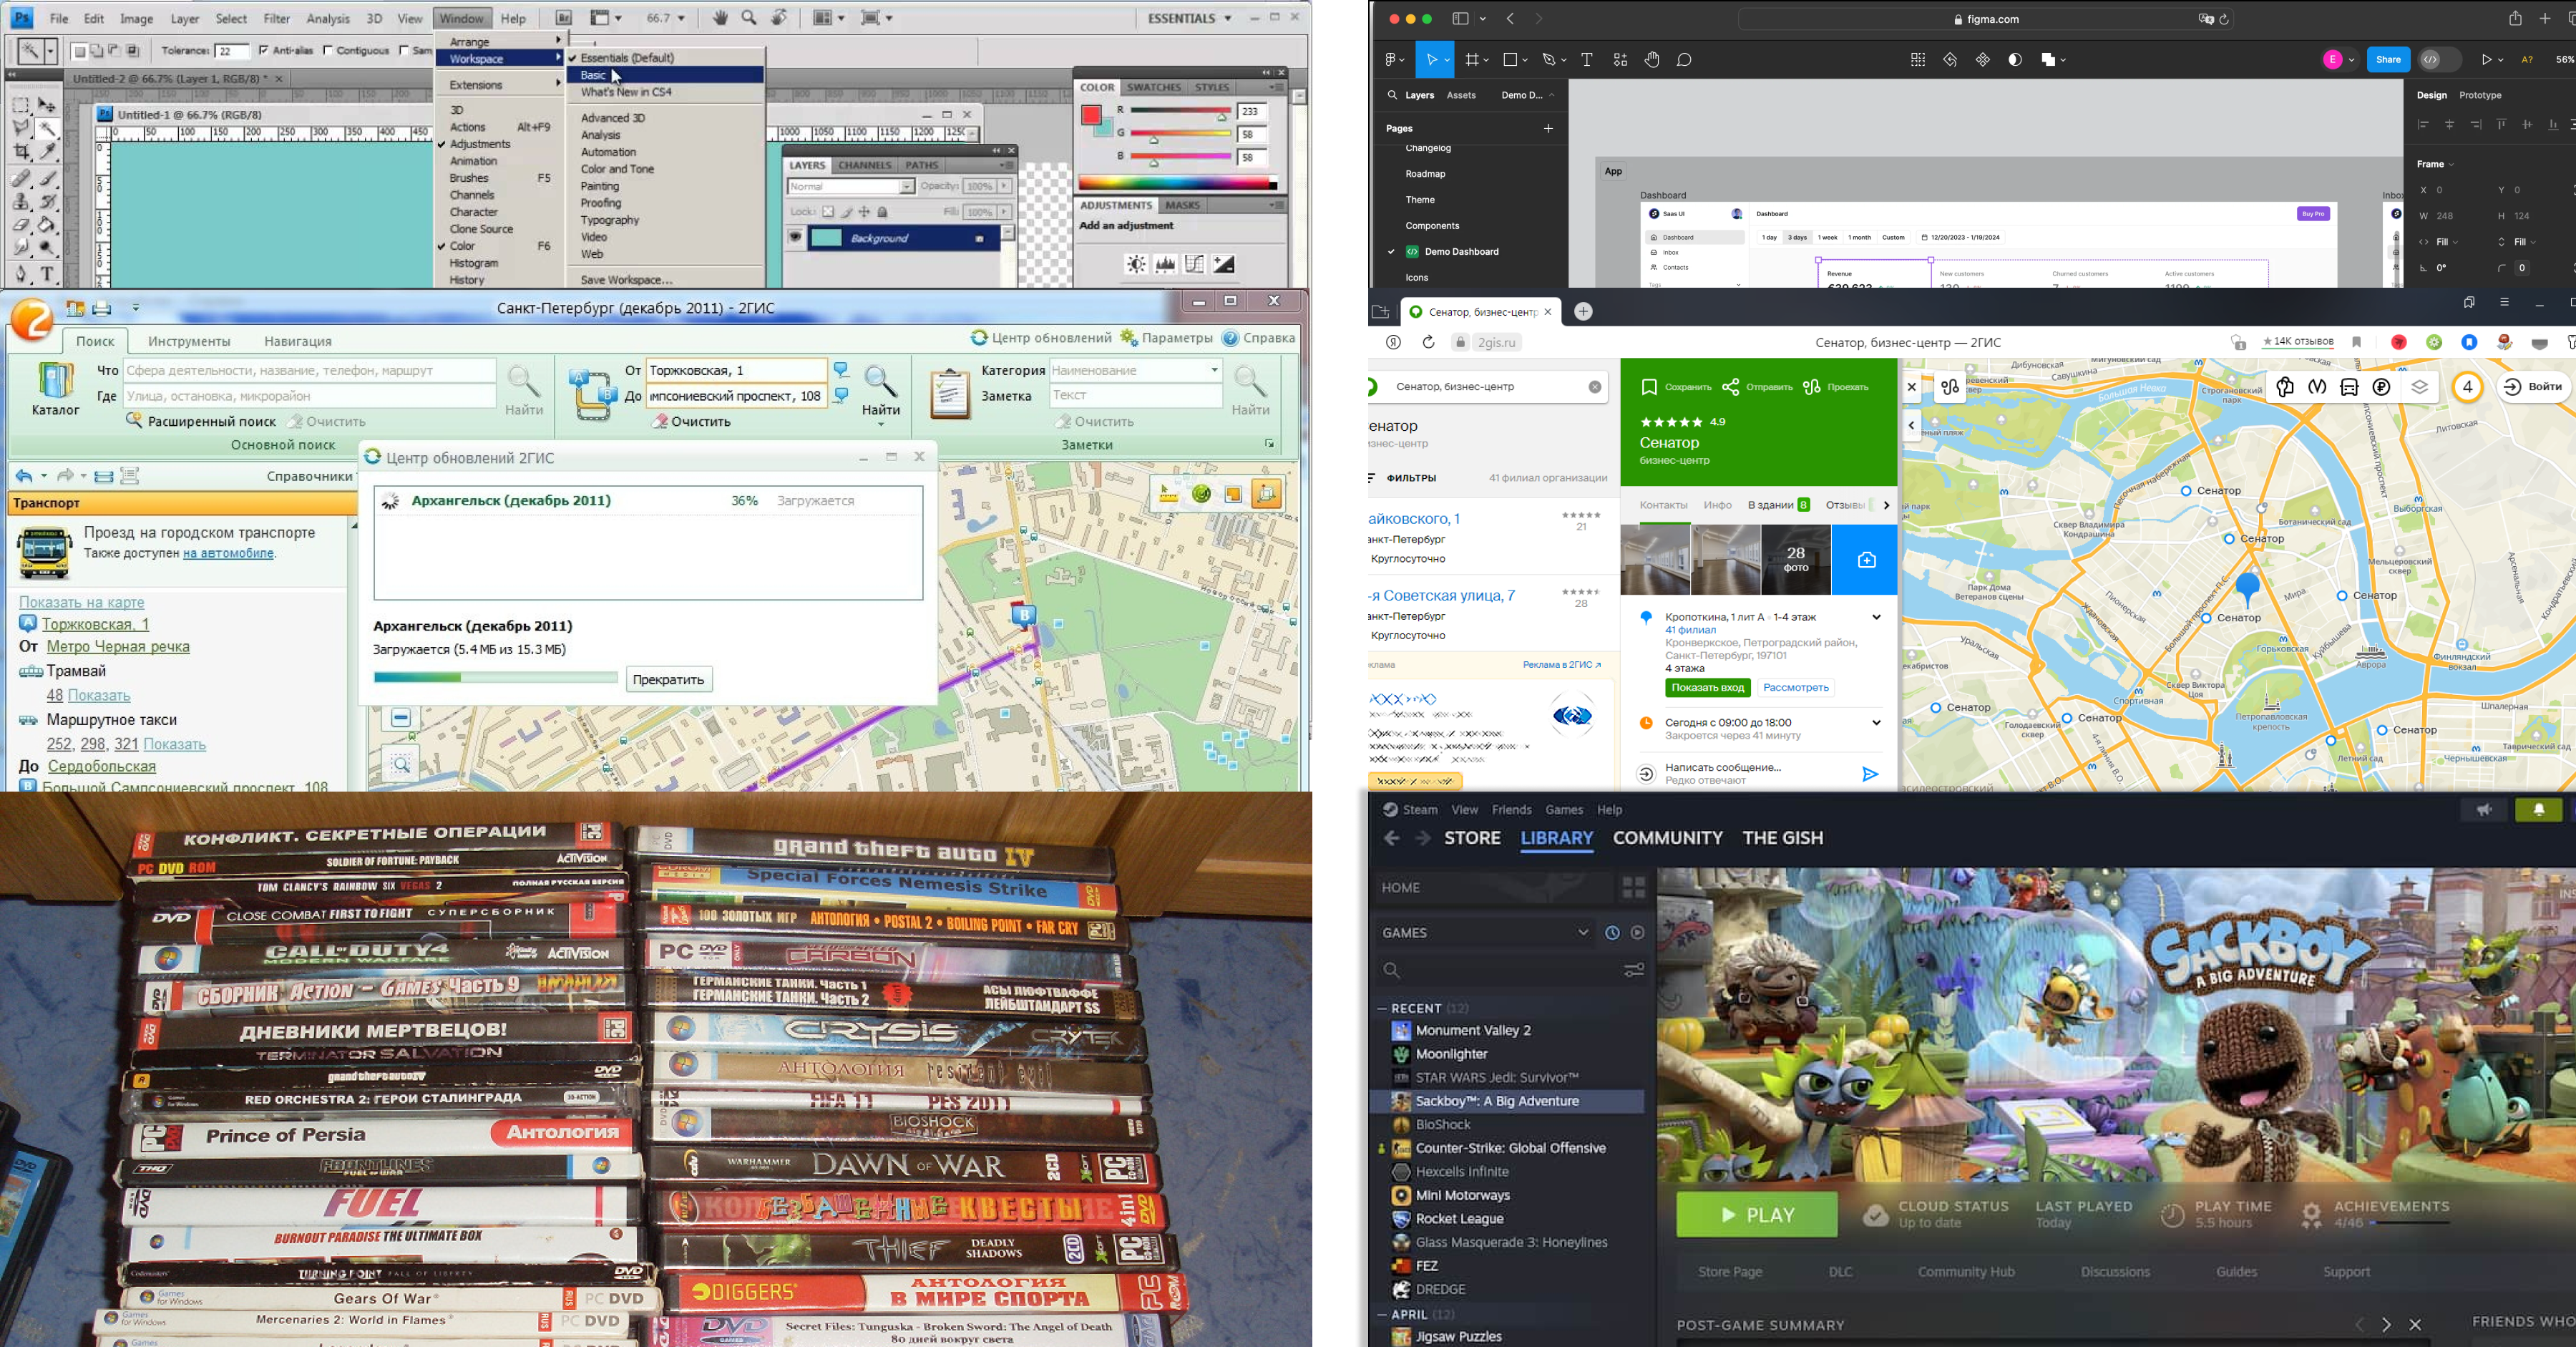
\includegraphics[width=0.8\textwidth]{images/old-vs-new}
        \end{figure}
    \end{frame}

    \begin{frame}{Компания FooBar}
        Описание компании — отрасль, продукт, команда, доход, скорость релизов
        7 эпизодов из жизни компании
        пару слов о the three ways
    \end{frame}

    {
        \setbeamertemplate{frame footer}{
            \scriptsize\href{https://example.com}{\textcolor{lightgray}{First Way}}
        }

        \begin{frame}{Эпизод 1. "Пятничный релиз️"}
            Контекст:
                Пятничный вечер. Разработичк Вася вручную заливает билд на прод с помощью SCP и запускает bash-скрипт,
                сохранившийся с прошлого релиза. Перед этим QA инженер Петя вручную проверил что все работает.
            Ситуация:
                Фича новая, протестирована вручную. Автотестов нет. В staging-среде билд собирали на локальной машине Васи.
                Сразу после релиза пользователи начинают жаловаться на падения и баги. Rollback невозможен — последняя копия
                стабильной версии лежит у Васи на ноутбуке, а он уже ушёл.
            Проблемы:
                Нет CI/CD, всё вручную
                Нет автоматических проверок
                Нет контроля версий билдов
                Вся надежда — на “память человека”
        \end{frame}

        \begin{frame}{Эпизод 2. “А staging у нас другой”}
            Контекст:
                После предыдущего инцидента внедрили автосборку и установку, а также разделили роли: Dev — сборка и тесты, Ops — обновление и дежурство.
                Команда выкатала новую фичу видеофильтров. На staging — всё идеально. После релиза — на проде звук тихий, а видео тормозит.
            Ситуация:
                Dev ставила новую версию на тестовые сервера с помощью одного скрипта, а Ops с помощью своего - из-за этого версии
                пакетов оказались разные.
            Проблемы:
                Среды staging ≠ production
                Нет описания инфраструктуры как кода
                Автотесты не покрывают окружение
                Нет среды, которая повторяет прод
                После проблем из кейса 1 была написана автоматизация, но фрагментарная: своя у Dev, своя у Ops
        \end{frame}
    }

    {
        \setbeamertemplate{frame footer}{
            \scriptsize\href{https://example.com}{\textcolor{lightgray}{Second Way}}
        }

        \begin{frame}{Эпизод 3: “Я же просто код пишу”}
            Контекст:
                Разработчик Вася добавил новую функцию сохранения видео в высоком качестве. При этом Вася не сообщил Ops о
                дополнительном использовании дискового пространства.
            Ситуация:
                Через пару дней на сервере закончилось место, из-за чего упали критичные сервисы. Ops не были готовы к резкому росту нагрузки.
            Проблемы:
                Отсутствие коммуникации между Dev и Ops
                Нет оценки влияния новых функций на инфраструктуру
                Нет мониторинга ресурсов и предупреждений
        \end{frame}

        \begin{frame}{Эпизод 4.  "Нагрузка растёт — и что?}
            Контекст:
                Фича “авто-превью видео” радует команду — красиво, удобно. Но пользователи жалуются на лаги. На проде — нагрузка выросла в 10 раз, CPU — 100%.
            Ситуация:
                Dev не замерял производительность, на staging данных было мало. Инфраструктура не выдерживает.
            Проблемы:
                Нет измерения производительности
                Нет метрик, профайлеров, логов
                Нет осознания “цены” кода
        \end{frame}

        \begin{frame}{Эпизод 5: “Фича умерла до релиза”}
            Контекст:
                Разработчик сделал фичу “рекомендации по интересам” — всё готово за 3 дня. Релиз — через 5 недель. За это время поменялся продуктовый приоритет.
            Ситуация:
                Сначала долгое ручное тестирование, потом согласования с безопасностью, потом очередь на релиз. За это время Dev успел забыть, как работает код.
            Проблемы:
                Длинный цикл разработки
                Ручные процессы
                Нет быстрой обратной связи
                Фича неактуальна на момент выхода
        \end{frame}
    }

    {
        \setbeamertemplate{frame footer}{
            \scriptsize\href{https://example.com}{\textcolor{lightgray}{Third Way}}
        }

        \begin{frame}{Эпизод 6. Случайный дроп БД на проде. Поиск виноватых}
            Контекст:
                Ночью после релиза прод перестал отвечать. Оказалось, что при миграции Dev случайно дропнул таблицу users, думая, что работает в тестовой базе.
            Реакция:
                Backup устарел. Ответственного нет — никто не проверил скрипт. Логи отсутствуют. Команда в панике ищет виноватого,а после того как нашли - публично отчитывают.
            Проблемы:
                Нет процессов ревью миграций
                Нет безопасных сред
                Нет культуры post-mortem
                Поиск “виноватого” вместо анализа
        \end{frame}

        \begin{frame}{Эпизод 7. Dev команда не пишет документацию к приложению}
            Контекст:
                Новая фича “режим обучения” готова. Dev уходит в отпуск. QA не знает, как тестировать.
                Ops не знает, как настроить конфигурациючтобы новая фича заработала. Менеджер не понимает как пользоваться
                новой функцией.
            Проблемы:
                Нет документации
                Знание в головах
                Команды изолированы
                Зависимость от конкретного человека
        \end{frame}
    }

    \begin{frame}{DevOps - это ...}
        - Итог всех кейсов. (Например: "Мы рассмотрели несколько кейсов, каждый из которых показывает типичную проблему в
        современных ИТ-командах: изолированность, фрагментация процессов, недостаток обратной связи, культура страха и
        отсутствия обучения.")
        - Формулировка "DevOps - это ...".
    \end{frame}

    \begin{frame}{Ключевые практики DevOps}
        \begin{itemize}
            \item CI/CD
            \item Infrastructure as Code (IaC), \href{https://www.cloudbees.com/blog/what-is-everything-as-code-eac\#why-should-you-adopt-everything-as-code}{Everything as Code (EaC)}
            \item Monitoring, Observability
            \item Культура сотрудничества: shared responsibility, blameless postmortems
        \end{itemize}
    \end{frame}

    \begin{frame}{DevOps инженер}
        - DevOps инженер существует
        - Почему возник DevOps инженер?
        - Какое место занимает DevOps инженер в современной разработке ПО?
    \end{frame}

    \begin{frame}{Заключение}
        - DevOps - это ...; Привести работы по теме "Что такое DevOps"
        - Актуальность DevOps
    \end{frame}

    \begin{frame}{Ссылки по теме}
        \begin{itemize}
            \item Ссылка 1
            \item Ссылка 2
        \end{itemize}
    \end{frame}
\end{document}

